\documentclass[12pt,a4paper,twoside,openright,titlepage,final]{article}
\usepackage{fontspec}
\usepackage{amsmath}
\usepackage{amsfonts}
\usepackage{amssymb}
\usepackage{makeidx}
\usepackage{graphicx}
\usepackage[hidelinks,unicode=true]{hyperref}
\usepackage[spanish,es-nodecimaldot,es-lcroman,es-tabla,es-noshorthands]{babel}
\usepackage[left=3cm,right=2cm, bottom=4cm]{geometry}
\usepackage{natbib}
\usepackage{microtype}
\usepackage{ifdraft}
\usepackage{verbatim}
\usepackage[obeyDraft]{todonotes}
\ifdraft{
	\usepackage{draftwatermark}
	\SetWatermarkText{BORRADOR}
	\SetWatermarkScale{0.7}
	\SetWatermarkColor{red}
}{}
\usepackage{booktabs}
\usepackage{longtable}
\usepackage{calc}
\usepackage{array}
\usepackage{caption}
\usepackage{subfigure}
\usepackage{footnote}
\usepackage{url}
\setsansfont[Ligatures=TeX]{texgyreadventor}
\setmainfont[Ligatures=TeX]{texgyrepagella}

%*******************************************************
%                 NO MODIFICAR
\newcommand*{\FSfont}[1]{%
  \fontencoding{T1}\fontfamily{#1}\selectfont}

\newlength{\tpheight}\setlength{\tpheight}{0.9\textheight}
\newlength{\txtheight}\setlength{\txtheight}{0.9\tpheight}
\newlength{\tpwidth}\setlength{\tpwidth}{0.9\textwidth}
\newlength{\txtwidth}\setlength{\txtwidth}{0.9\tpwidth}
\newlength{\drop}
%*******************************************************

% Crea una portada con los siguientes parámetros
%
% #1 : Título 
% #2 : Subtítulo
% #3 : Subsubtítulo
% #4 : Autor(es)
% #5 : Lugar
%

\newcommand*{\portada}[5]{
\begin{titlepage}
\begingroup
\vspace*{1cm}
\drop = 0.2\txtheight
\centering
\vfill
{\Huge \scshape #1}\\[\baselineskip]
{\Large \textbf{#2}}\\[\baselineskip]
{\Large \scshape #3}\\[\baselineskip]
\vspace*{0.3cm}
{\large \textit{#4}}\\[0.5\drop]

\includegraphics[scale=0.35]{./imagenes/logoURJC.jpg}
\vspace*{1.5cm}

{\large \scshape #5, \today} \par
\begin{center}
\end{center}
\vfill\null
\endgroup
\end{titlepage}
}
 %*****************************************************
 


\author{José Ignacio Escribano}

\title{Caso práctico I}

\setlength{\parindent}{0pt}

\begin{document}

\pagenumbering{alph}
\setcounter{page}{1}

\portada{Caso Práctico I}{Modelización y tratamiento de la incertidumbre}{Estadística descriptiva}{José Ignacio Escribano}{Móstoles}

\listoffigures
\thispagestyle{empty}
\newpage

\tableofcontents
\thispagestyle{empty}
\newpage


\pagenumbering{arabic}
\setcounter{page}{1}

\section{Introducción}

Para la realización de este caso práctico requerimos dos conjuntos de datos: un conjunto cuantitativo discreto y otro cuantitativo continuo. Cuando dispongamos de estos conjuntos de datos procederemos a realizar un análisis descriptivo de cada uno de éstos.\\

Para ello, necesitamos encontrar una base de datos que disponga de los conjuntos de datos requeridos anteriormente. La base de datos elegida se centra en el estudio de la liga norteamericana de béisbol de la temporada 1986. Los datos se encuentran disponibles en el siguiente enlace: \url{http://lib.stat.cmu.edu/datasets/baseball.data}\footnote{El archivo se encuentra en forma de ``shell archive'', que es una forma de fichero autoextraíble, en el que se agrupan varios archivos, tanto de datos como descripciones de las variables. Para poder extraer estos ficheros, ejecutaremos en una terminal el comando \textbf{sh} seguido del nombre del fichero. Esto creará cuatro ficheros nuevos: \textit{pitcher.final}, \textit{team.final}, \textit{data.des.form}, \textit{hitter.final}. De estos ficheros sólo nos interesan los dos últimos: en el primero se encuentran las descripciones de las variables; y en el segundo, los datos que utilizaremos para nuestro análisis descriptivo.}. En el archivo se encuentran distintos datos relativos a equipos, pitchers y hitters. Nos centraremos en estos últimos. De entre las $24$ variables disponibles en el fichero utilizaremos como variable cuantitativa discreta el número de homeruns durante la temporada 1986, y como variable cuantitativa continua el salario (en miles de dólares) al comienzo de la temporada 1987.  

\section{Análisis descriptivo de un conjunto de datos cuantitativos discretos}

El conjunto de datos cuantitativo discreto elegido es \textbf{el número de homeruns de los ``hitters'' de la liga norteamericana de béisbol durante la temporada 1986}.\\

Para realizar el análisis descriptivo de este conjunto de datos, realizaremos distintos tipos de gráficos como el gráfico de barras y sectores, entre otros. Posteriormente, daremos una serie de medidas, tanto de centralización, posición como de dispersión.\\

Comencemos realizando el diagrama de barras para ver como se distribuye la frecuencia de cada uno de los posibles valores de la variable número de homeruns. En la Figura~\ref{fig:diagrama_barras_homeruns} se muestra este diagrama. Se puede observar que la frecuencia se mantiene más o menos constante entre los $0$ y $9$ homeruns, mientras que a partir de $10$, la frecuencia desciende de manera considerable. Y la realización de $31$ homeruns o más es bastante infrecuente.\\

\begin{figure}[tbph!]
\centering
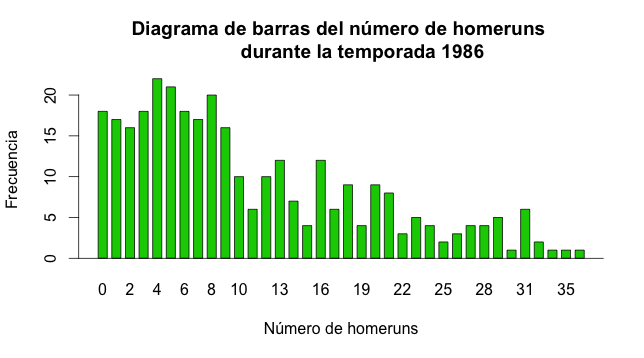
\includegraphics[width=0.8\linewidth]{imagenes/diagrama_barras_homeruns}
\caption{Diagrama de barras para el número de homeruns}
\label{fig:diagrama_barras_homeruns}
\end{figure}

Si realizamos el diagrama de sectores (Figura~\ref{fig:diagrama_sector_homeruns}), veremos que el número de posibles valores es $41$: desde $0$ hasta $40$ homeruns, que es el máximo. Debido a este gran número de valores, el gráfico no se aprecia bien.\\

\begin{figure}[tbph!]
\centering
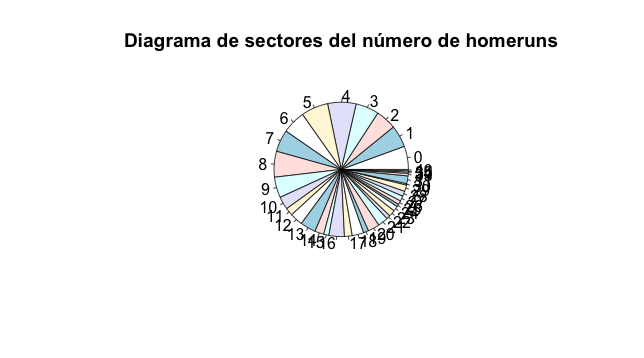
\includegraphics[width=\linewidth]{imagenes/diagrama_sectores_homeruns}
\caption{Diagrama de sectores para el número de homeruns}
\label{fig:diagrama_sector_homeruns}
\end{figure}

Para asegurarnos de que lo visto en los gráficos anteriores se corresponde con la realidad de los datos, calcularemos una serie de medidas de distintos tipos: de centralización, de posición y de dispersión. \\

Las medidas de centralización que consideraremos son la media aritmética, la mediana y la moda. Estas medidas son:

\begin{table}[htbp]
\centering
\begin{tabular}{|c|c|}
\hline Media & 10.77019 \\ 
\hline Mediana & 8 \\ 
\hline Moda & 4  \\ 
\hline 
\end{tabular} 
\end{table}

La media y la mediana son bastante parecidas, por lo que se puede suponer que son medidas representativas de los datos. Sin embargo, la moda está muy alejada de las otras dos medias, pero este valor es el más frecuente de nuestro conjunto de datos.\\


Las medidas de posición que consideraremos serán los cuartiles y los deciles. Entre los primeros, optaremos por el primer ($Q_1$) y el tercer cuartil ($Q_3$); y de los segundos, optaremos por el segundo ($D_2$) y el noveno decil ($D_{9}$). \\

\begin{table}[htbp]
\centering
\begin{tabular}{|c|c|}
\hline $Q_1$ & 4 \\ 
\hline $Q_3$ & 16 \\ 
\hline $D_2$& 3  \\ 
\hline $D_9$& 24  \\ 
\hline 
\end{tabular} 
\end{table}

De los cuartiles $Q_1$ y $Q_3$ concluimos que el $25\%$ de los jugadores consiguen $4$ o menos homeruns y que el $75 \%$ de los jugadores hacen $16$ homeruns o menos. De la misma forma, el $20\%$ de los jugadores consiguen menos de $3$ homeruns; y el $90\%$ hace $24$ o menos homeruns.\\

Las medidas de dispersión que utilizaremos son la varianza y la cuasivarianza, la desviación estándar, el rango y el rango intercuartílico.\\

\begin{table}[htbp]
\centering
\begin{tabular}{|c|c|}
\hline Varianza & 75.61178 \\ 
\hline Cuasivarianza & 75.84733 \\
\hline Desviación estándar & 8.709037 \\  
\hline Rango & 40  \\ 
\hline Rango intercuartílico & 12  \\ 
\hline 
\end{tabular} 
\end{table}

De los resultados anteriores vemos que la varianza es muy elevada, lo que hace que haya gran variabilidad de los datos. El rango también es muy grande debido a todos los posibles valores que toman los datos: entre $0$ y $40$. Si aplicamos la desigualdad de Chebyshev, con $k = 3.16$, tenemos que al menos el 90\% de los datos se encuentran en el intervalo $(-16.72, 38.26)$. Puesto que no tenemos ningún valor menor que cero, podemos decir que al menos el 90\% de los datos se encuentran en el intervalo $[0, 38.26)$.\\

Con el rango intercuartílico podemos obtener el diagrama de cajas (Figura~\ref{fig:diagrama_cajas_homeruns}). Podemos observar que el rango intercuartílico se sitúa entre $4$ y $16$ homeruns y la mediana es de $8$ homeruns. Hay que destacar que hay dos datos atípicos, por lo que conseguir $35$ ó $40$ homeruns es poco común en los jugadores de la temporada 1986.\\

\begin{figure}[tbph!]
\centering
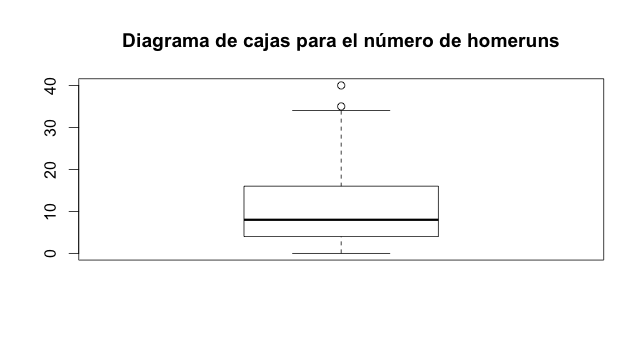
\includegraphics[width=0.8\linewidth]{imagenes/diagrama_cajas_homeruns}
\caption{Diagrama de cajas para el número de homeruns}
\label{fig:diagrama_cajas_homeruns}
\end{figure}

Por último, calculamos las medidas de asimetría y el curtosis. Los datos se muestran a continuación:

\begin{table}[htbp]
\centering
\begin{tabular}{|c|c|}
\hline Asimetría & 0.8963904 \\ 
\hline Curtosis & 0.001943684 \\
\hline 
\end{tabular} 
\end{table}

Puesto que el coeficiente de asimetría es mayor que cero, tenemos asimetría a la derecha. Con respecto al curtosis, tenemos una distribución de los datos casi normal ya es práctica cero.

\newpage 

\section{Análisis descriptivo de un conjunto de datos cuantitativos continuos}

El conjunto de datos continuo elegido es \textbf{el salario (en miles de dólares) de los ``hitters'' al comienzo de la temporada 1987}. De igual modo que en el caso discreto, daremos distintos gráficos y distintas medidas para realizar el análisis descriptivo.\\

Si echamos un vistazo a este conjunto de datos, veremos que hay datos que no están disponibles (se muestran como \textit{NA}), por lo que debemos eliminarlos a la hora de realizar el análisis descriptivo.\\

Comencemos, de nuevo, representando los datos mediante una serie de gráficos. En este caso, utilizaremos un histograma y un gráfico de tallos y hojas.\\

El histograma (Figura~\ref{fig:histograma_salario}) muestra que el salario más frecuente se encuentra entre $0$ y $200$ miles de dólares. Según va aumentando el salario, la frecuencia va disminuyendo, hasta el máximo que se encuentra en torno a $2500$ miles de dólares, que es muy poco frecuente.\\ 

\begin{figure}[tbph!]
\centering
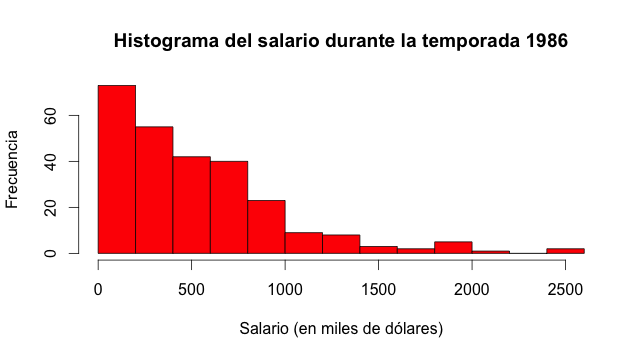
\includegraphics[width=0.8\linewidth]{imagenes/histograma_salario}
\caption{Histograma para el salario}
\label{fig:histograma_salario}
\end{figure}

El diagrama de tallos y hojas se puede ver a continuación:

\begin{verbatim}
   0 | 7777777888888999999999
   1 | 0000000011111122233444444
   1 | 555566666777888889999
   2 | 00000011222333444
   2 | 5555555567888889
   3 | 00000012333444
   3 | 555677899
   4 | 000022233333
   4 | 55555888899
   5 | 00001233344
   5 | 5556889
   6 | 0000013334
   6 | 56678
   7 | 0000013344444
   7 | 555555557788889
   8 | 0023
   8 | 55558888
   9 | 0002334
   9 | 556
  10 | 000144
  10 | 5
  11 | 0
  11 | 588
  12 | 024
  12 | 6
  13 | 0001
  13 | 5
  14 | 
  14 | 5
  15 | 0
  15 | 
  16 | 0
  16 | 7
  17 | 
  17 | 
  18 | 0
  18 | 6
  19 | 034
  19 | 8
  20 | 
  20 | 
  21 | 3
  21 | 
  22 | 
  22 | 
  23 | 
  23 | 
  24 | 1
  24 | 6

\end{verbatim}

Como en el caso discreto, calcularemos una serie de medidas, que serán de centralización, de posición y de dispersión.\\

En el caso de las medidas de centralización utilizaremos la media y la mediana. Los resultados se pueden ver a continuación:\\

\begin{table}[htbp]
\centering
\begin{tabular}{|c|c|}
\hline Media & 535.9259 \\ 
\hline Mediana & 425 \\ 
\hline 
\end{tabular} 
\end{table}

Vemos que tanto la mediana como la media están bastante distantes la una de la otra, por lo que podemos considerar que la medida más representativa de nuestro conjunto de datos es la mediana, que deja tanto a su izquierda como a su derecha un 50\% de los datos.\\

Las medidas de posición que consideraremos serán los cuartiles y los deciles: de los primeros elegiremos el primero ($Q_1$) y el tercero ($Q_3$); y de los segundos, el segundo ($D_2$) y el noveno decil ($D_9$). Los datos se muestran a continuación:\\

\begin{table}[htbp]
\centering
\begin{tabular}{|c|c|}
\hline $Q_1$ & 190 \\ 
\hline $Q_3$ & 750 \\ 
\hline $D_2$& 155  \\ 
\hline $D_9$& 1048.667  \\ 
\hline 
\end{tabular} 
\end{table}

Podemos decir que el $25\%$ de los jugadores cobró $190$ o menos, y el $75\%$ cobró $750$ o menos. De igual forma, con los deciles, podemos decir que el $20\%$ cobraba menos de $155$ y el $90\%$ cobró menos de $1048.667$.\\

Las medidas de dispersión que utilizaremos son la varianza y la cuasivarianza, la desviación estándar y el rango y el rango intercuartílico. Los datos se muestran a continuación:

\begin{table}[htbp]
\centering
\begin{tabular}{|c|c|}
\hline Varianza & 202734.3 \\ 
\hline Cuasivarianza & 203508.1 \\
\hline Desviación estándar & 451.1187 \\  
\hline Rango & 2392.5  \\ 
\hline Rango intercuartílico & 560  \\ 
\hline 
\end{tabular} 
\end{table}

Vemos que existe una gran varianza, por lo que existe una gran dispersión de los datos, que comprobamos mirando el rango, que es muy amplio. Con todos estos datos representamos el diagrama de cajas (Figura~\ref{fig:diagrama_cajas_salario}). En él se muestra que el rango intercuartílico se sitúa entre $190$ y $750$. También observamos que existen una gran cantidad de datos atípicos, por lo que encontrar jugadores que cobraran entre $1500$ y $2500$ al comienzo de la temporada 1987 era bastante infrecuente. Si aplicamos la desigualdad de Chebyshev, con $k = 3.16$, tenemos que al menos el 90\% de los datos se encuentran en el intervalo $(-88958, 1961.42)$. Como no existen salarios menores que cero, podemos decir que al menos el 90\% de los datos se encuentran en el intervalo $[0, 1961.42)$.\\

\begin{figure}[tbph!]
\centering
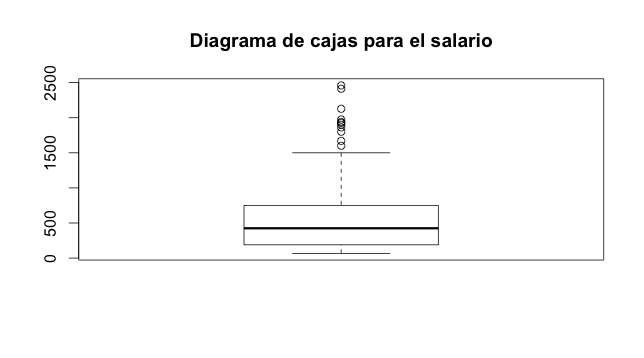
\includegraphics[width=0.8\linewidth]{imagenes/diagrama_cajas_salario}
\caption{Diagrama de cajas para el salario}
\label{fig:diagrama_cajas_salario}
\end{figure}

Por último, calculamos las medidas de asimetría y el curtosis. Los datos se muestran a continuación:

\begin{table}[htbp]
\centering
\begin{tabular}{|c|c|}
\hline Asimetría & 1.570888 \\ 
\hline Curtosis & 2.933014 \\
\hline 
\end{tabular} 
\end{table}

Puesto que el coeficiente de asimetría es mayor que cero, tenemos asimetría a la derecha. Con respecto al curtosis, tenemos una distribución de los datos leptocúrtica. 


\section{Conclusiones}

En este caso práctico hemos visto cómo realizar tanto un análisis descriptivo para una variable discreta como para una variable continua. Tanto los gráficos como las medidas nos han dado una serie de interpretaciones acerca de los datos. Por último, hemos aprendido a utilizar de forma básica el lenguaje de programación R, un lenguaje muy potente utilizado en multitud de situaciones.

\newpage

\section{Código R}

\verbatiminput{../caso_i.R}


\end{document}




 